\section{Anforderungen und Auslegungskriterien}
In diesem Kapitel wird beschrieben, welchen Anforderungen der Solar Butterfly und dessen Komponenten gerecht werden müssen. In einem ersten Schritt wird auf die allgemeinen Anforderungen des Solar Butterflys und anschliessen auf die daraus resultierenden Auslegungskriterien der einzelnen Komponenten eingegangen. Es wird beschrieben, was die Anforderungen konkret für die einzelnen Komponenten bedeuten und wie gewährleistet werden kann, dass diese erfüllt werden.\\
Weiter werden  Design-Allowables festgelegt und erläutert, wie gedenkt wird, die Problematik der Ermüdung	anzugehen.


\subsection{Anforderungen an den Solar Butterfly}
Im Rahmen dieser Arbeit wird lediglich auf diejenigen Anforderungen des Solar Butterflys eingegangen, welche für die Auslegung der Grundstruktur und den Festigkeitsberechnungen relevant sind. Die komplette Liste der Anforderungen an den Solar Butterfly ist in der Arbeit von \emph{Huber} \cite{Huber} oder im elektronischen Anhang \ref{e:Anforderungsliste} zu finden.\\
Was nun folgt, sind diejenigen Anforderungen, welche in dieser Arbeit von Relevanz sind und genauer betrachtet werden.

\begin{itemize}
  \item Der Solar Butterfly muss strukturelle Integrität aufweisen. Dies bedeutet, dass die Struktur des Solar Butterflys den vorgesehenen Belastungen (vgl. Lastenheft Kapitel \ref{Lastenheft}) standhalten muss, ohne dabei durch Bruch, Fliessen, Verformung oder Ermüdung zu versagen.
  \item Weiter darf der Solar Butterfly sich nicht so stark deformieren, dass seine Funktionstauglichkeit eingeschränkt wird. Die konkreten Anforderungen an die Deformierbarkeit der einzelnen Komponenten des Solar Butterflys werden bei deren Auslegung genauer betrachtet und beschrieben.
  \item \emph{Palmer} will mit dem Solar Butterfly ein nachhaltiges und langlebiges Produkt entwickeln, was umgesetzt wird in dem eine \emph{Safe-Life-Quality} in der Auslegung angestrebt wird, welche \glqq die absolute Schadensfreiheit für das ganze Leben\grqq{} verlangt \cite{klein}.
\end{itemize}

\subsection{Dauerfestigkeit}
Die Anforderung an die Langlebigkeit des Solar Butterflys wird erfüllt, indem dieser Dauerfest ausgelegt wird. Für die Grobauslegung bedeutet dies konkret, dass die Ermüdung mit einer entsprechenden Wahl der Design-Allowables pauschal abgedeckt wird und dass Spannungserhöhungen mit gutem Design vermieden werden.\\
Als Dauerbelastung wird vereinfacht angenommen, dass die maximalen Lasten zu 50\% (die Hälfte der Amplitude) dauerhaft auftreten. Dies bedeutet, anders formuliert, dass angenommen wird, dass die im Lastenheft definierten maximalen Lasten selten zu 50\% erreicht werden und dass diese somit keine Gefahr für das Versagen der Bauteile durch Ermüdung darstellen.\\
Ob dies eine angemessene Annahme ist, muss zu einem späteren Zeitpunkt und bei einem weiter fortgeschrittenen Projektstand, durch Erbringung eines Nachweises der Dauerfestigkeit, überprüft werden.
\newpage

\subsection{Design-Allowables und Materialkennwerte}
Um den Prozess der Grobauslegung zu vereinfachen, werden sogenannte Design-Allowables definiert. Dies sind Materialkennwerte welche für die überschlägige Auslegung von Bauteilen verwendet werden können.\\
In der Tabelle \ref{tab:Design-Allowables} sind die Materialkennwerte und Design-Allowables der für die Deckschichten oder Profile verwendeten Materialien zusammengetragen. Da der Solar Butterfly für 50\% der Belastungen dauerfest ausgelegt wird und für die Auslegung der Dauerfestigkeit ein Sicherheitsfaktor von 2 verwendet wird, entsprechen die zulässigen Dauerfestigkeitswerte direkt auch der Dauerfestigkeiten der Materialien.
% Die Sicherheitsfaktoren wurden nach \emph{Roloff Matek Maschinenelemente} gewählt \cite{Roloff}.

%GFK: Roloff Matek S.1013
\begin{table}[H]
  \centering
  \caption{Design-Allowables für Materialien der Profile und Deckschichten}
  \begin{tabular}{llccccc}	\hline
    Werkstoff	&	Grösse	&		&	Einheit	&	Wert	&	$S_f$	&	Zulässig\\	\hline
    \multirow{5}{*}{Aluminium\cite{alu1}}	&	Dichte	&	$\rho$        	&	$\frac{kg}{m^3}$	&	2710	&		&		\\
      &	E-Modul	&	              	&	MPa	&	70'000	&		&		\\
      &	Zugfestigkeit	&	$\sigma$      	&	MPa	&	240	&	1.5	&	160	\\
      &	Wechselfestigkeit	&	$\sigma_{zdW}$	&	MPa	&	80	&	2	&	80	\\
      &	Biegewechselfestigkeit	&	$\sigma_{bW}$ 	&	MPa	&	100	&	2	&	100	\\	\hline
    \multirow{4}{*}{GFK\footnotemark\cite{Roloff}}	&	Dichte	&	$\rho$        	&	$\frac{kg}{m^3}$	&	1650	&		&		\\
      &	E-Modul	&	              	&	MPa	&	16'000	&		&		\\
      &	Zugfestigkeit	&	$\sigma$      	&	MPa	&	250	&	1.5	&	167	\\
      &	Biegewechselfestigkeit	&	$\sigma_{bW}$ 	&	MPa	&	50	&	2	&	50	\\	\hline
  \end{tabular}
  \label{tab:Design-Allowables}
\end{table}

\footnotetext[1]{Glasfaserverstärkter Kunststoff}

Für die Verklebung der Strukturelemente wurde noch kein definitiver Klebstoff ausgewählt. Als Anhaltspunkt wird der Klebstoff \emph{Sikaflex-552 AT} verwendet, welcher im Automobilbau Anwendungen findet und vom Sponsor des Chassis \emph{Geser Fahrzeugbau AG} häufig verwendet wird. Nach \emph{Roloff Matek Maschinenelemente} wird für Klebeverbindung mit unbekannten (oder nicht genau bekannten) Abminderungsfaktoren der Sicherheitsfaktor von 2.5 gewählt. Als Abminderungsfaktor wird, gemäss der Faustregel für dynamisch Beanspruchte Bindefestigkeiten von \emph{Habenicht} \cite{kleben1}, ein Wert von 0.1 gewählt.

\begin{table}[H]
  \centering
  \caption{Design-Allowables für Kleber}
  \begin{tabular}{llcccccc}	\hline
    Werkstoff	&	Grösse	&		&	Einheit	&	Wert	&	$S_f$	&	Abminderungsf.&	Zulässig	\\	\hline
    \multirow{3}{*}{Sikaflex-552 AT}	&	Dichte	&	$\rho$        	&	$\frac{kg}{m^3}$	&	1500	&		&		&		\\
      &	Schubfestigkeit	&	$\tau$	&	MPa	&	2	&	2.5	&	0.1	&	0.16	\\
      &	Zugfestigkeit	&	$\sigma$      	&	MPa	&	3	&	2.5	&	0.1	&	0.24	\\	\hline
  \end{tabular}
  \label{tab:Design-Allowables Kleben}
\end{table}

Das Materialdatenblatt des Klebstoffes ist im elektronischen Anhang \ref{e:Sikaflex} angefügt.
\newpage

\subsection{Auslegungskriterien}
In diesem Unterkapitel beschrieben, was die Anforderungen an den Solar Butterfly für die einzelnen Komponenten und Strukturelemente bedeutet. Es wird erläutert mit welchen Methoden die Auslegung angegangen wird und welche Vereinfachungen getroffen werden.

  \subsubsection{Aluminiumstrukturen}
  Zu den Auslegungskriterien der Aluminiumstrukturen gehört das Festigkeitsproblem der plastischen Verformung (Fliessen) und das Stabilitätsproblem der Knickung. Für die Grobauslegung werden die Aluminiumstrukturen ausgelegt, dass diese ein Sicherheitsfaktor gegen Fliessen von 1.5 aufweisen. Bei der Wahl dieses Sicherheitsfaktors wird sich an \emph{Roloff Matek Maschinenelemente} orientiert \cite{Roloff}. Für das Stabilitätsproblem der Knickung wird sich an \emph{Bärtsch} orientiert und ein Sicherheitsfaktor von 4 gewählt \cite{Baertsch}.

  \paragraph{Fliessen}\mbox{}\\
  Um die Sicherheit eines Strukturelementes gegen Fliessen zu gewährleisten, wird überprüft, ob die \emph{Von Mises}-Vergleichsspannung kleiner als die zulässige Spannung ist. Die \emph{Von Mises}-Vergleichsspannung kann gemäss der Formel \ref{Von Mises} berechnet werden \cite{Baertsch}.
  \begin{equation}
    \label{Von Mises}
    \sigma_v = \sqrt{\sigma_x^{2}-\sigma_x \cdot \sigma_y + \sigma_y^2 + 3\tau^2}
  \end{equation}

  \paragraph{Knicken}\mbox{}\\
  Das Knicken von Stäben wird abgedeckt, indem überprüft wird, ob die Knickspannung nach Euler die zulässige Spannung überschreitet. Knickspannung nach Euler:
  \begin{equation}
    \sigma_{zul} \leq \sigma_k = \frac{\pi^2 \cdot E \cdot I_{min}}{{l_k}^2 \cdot A}
  \end{equation}

  \subsubsection{Sandwichstrukturen}
  Die Versagenskriterien der Sandwichstrukturen können in die beiden Kategorien \emph{Festigkeitsprobleme} und \emph{Stabilitätsprobleme} eingeteilt werden \cite{ETH}. In der Abbildung \ref{Sandwich} sind die verschiedenen Versagensfälle dargestellt \cite{Sandwich}.

  \begin{center}
    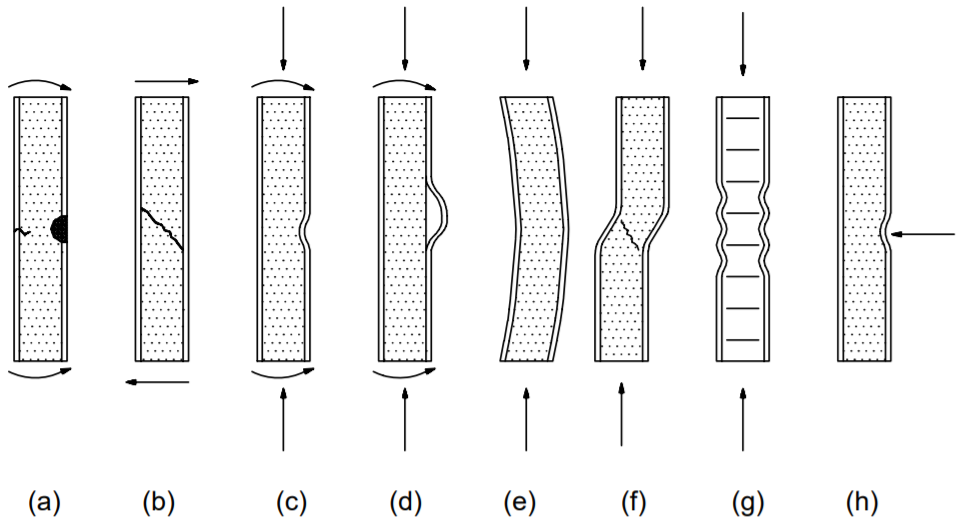
\includegraphics[width=0.65\textwidth]{04_Figures/Sandwich.png}
    \captionof{figure}{Versagensarten in Sandwichbalken.
                      (a) Fliessen/Bruch der Oberfläche,
                      (b) Schubbruch,
                      (c und d) Faltenbildung der Oberfläche,
                      (e) allgemeines Knicken,
                      (f) Scherfaltenbildung,
                      (g) Beulen an der Oberfläche und
                      (h) lokales Eindrücken.}
    \label{Sandwich}
  \end{center}

  Zu den Festigkeitsproblemen gehören;
  \begin{itemize}
    \item Fliessen der Deckschicht,
    \item Schubbruch der Kernschicht,
    \item Delamination und
    \item Ermüdung.
  \end{itemize}

  Zu den Stabilitätsproblemen gehören unteranderem;
  \begin{itemize}
    \item Knickung,
    \item Schubbeulung der Kernschicht (Shear Crimping) und
    \item Kurzwelliges Beulen der Deckschicht (Wrinkling).\\
  \end{itemize}

  Die auszulegenden Sandwichstrukturen werden gegenüber diesen Festigkeits und Stabilitätsproblemen ausgelegt.\\
  Um den Rechenaufwand und die Komplexität der Berechnungen zu verringern werden Annahmen und Vereinfachungen getroffen. Für die Auslegung von Sandwichstrukturen können folgende Annahmen getroffen werden \cite{klein}\cite{ETH};
  \begin{itemize}
    \item linear elastische und isentrope Materialverhalten,
    \item Eigenbiegesteifigkeiten der Deckschichten sind vernachlässigbar,
    \item Dehnsteifigkeit der Kernschicht ist vernachlässigbar und
    \item die Kernschicht lässt sich nicht zusammendrücken.\\
  \end{itemize}
  Aus den getroffenen Annahmen resultiert ein vereinfachter Spannungszustand, welcher besagt, dass die Deckschichten jeweils die Normalkräfte und die Kernschichten die Schubkräfte aufnehmen. (Sandwichmembrantheorie)

    \paragraph{Festigkeitsprobleme}\mbox{}\\
    Aus den getroffenen Annahmen und Vereinfachungen lassen sich die Formeln \ref{Spannung in Deckschicht} und \ref{Schubspannungen im Kern} herleiten. Mit der Formel \ref{Spannung in Deckschicht} lassen sich die Spannungen in den Deckschichten berechnen.

    \begin{equation}
      \label{Spannung in Deckschicht}
      \sigma_d = \frac{1}{t_d}\cdot \left ( \frac{n}{2} \pm \frac{m}{h}\right )
    \end{equation}

    Wobei $t_d$ für die Dicke der Deckschicht, $n$ für die Normalkraft pro Länge, $m$ für das Moment pro Länge und $h$ für die rechnerische Höhe der Platte stehen.

    Mit der Formel \ref{Schubspannungen im Kern} lassen sich die Schubspannungen in der Kernschicht berechnen und somit Aussagen über ihre Resistenz gegenüber dem Schubbruch machen.
    \begin{equation}
      \label{Schubspannungen im Kern}
      \tau_k = \frac{q}{t_k}
    \end{equation}

    Wobei $t_k$ für die Dicke der Kernschicht steht.

    Die Delamination der Deckschichten wird abgesichert, indem die Auswahl des Klebers, oder im Falle einer Laminierung die Wahl des Matrixwerkstoffes, so getroffen wird, dass dieser eine höhere Schubfestigkeit aufweist als das Material der jeweiligen Kernschicht.

    \paragraph{Stabilitätsprobleme}\mbox{}\\
    Die Stabilitätsprobleme der Sandwichstrukturen lassen sich in globale und lokale Instabilitäten einteilen. Zur globalen Instabilität gehört das Knicken, welches sich aus der Euler-Knickung des schubsteifen Balkens und dem Schubknicken zusammensetzt. Die kritische Belastung, bei welcher es zur Euler-Knickung kommt, lässt sich gemäss \emph{Klein} \cite{klein} mit der Formel \ref{Euler-Knicklast} berechnen.

    \begin{equation}
      \label{Euler-Knicklast}
      F_{kB}=\frac{\pi^2 \cdot E_d \cdot I}{l_k^{2}}
    \end{equation}

    Wobei sich das Widerstandsmoment $I$ vereinfacht gemäss der Formel \ref{ID} berechnen lässt. Hier wurde die Annahme getroffen, dass die Eigenbiegesteifigkeiten der Deckschichten vernachlässigbar sind. Diese Annahme kann gemäss \emph{Klein} ab einem Verhältnis von $t_d$ zu $t_k$ von 0.25, getroffen werden.
    \begin{equation}
      \label{ID}
      I= 2 \cdot b \cdot t_d \cdot \left( \frac{t_k}{2} + t_d \right )^{2}
      % B_y = 2\cdot b \cdot t_d\cdot \left ( \frac{t_k}{2}+t_d \right )^2
    \end{equation}

    Die kritische Schubknicklast lässt sich gemäss \emph{Klein} mit der Formel \ref{Schubknicklast} berechnen.
    \begin{equation}
      \label{Schubknicklast}
      F_{kS} = b \cdot t_k \cdot G_k
    \end{equation}

    Die totale kritische Knicklast \(F_k\) ergibt sich aus der Formel \ref{Knicklast}:
    \begin{equation}
      \label{Knicklast}
      F_{k, vorh.} \leq F_k=\frac{1}{\frac{1}{F_{kB}}+\frac{1}{F_{kS}}}
    \end{equation}

    Zu den lokalen Instabilitäten zählen das Schubbeulen und das Knittern der Deckschicht. Die kritischen Spannungen, bei welcher Schubbeulen auftritt, lässt sich aus den Formel \ref{Schubbeulen} berechnen. \cite{ETH}
    \begin{equation}
      \label{Schubbeulen}
      \sigma_k = G_k \cdot \frac{h}{2 \cdot t_d}
    \end{equation}

    Die kritischen Spannungen, bei welcher das Knittern der Deckschicht auftritt, lässt sich mit der Formel \ref{Knittern} berechnen. \cite{ETH}
    \begin{equation}
      \label{Knittern}
      \sigma_k = k_s\sqrt[3]{E_d \cdot E_k \cdot G_k}
    \end{equation}
    Wobei für Auslegungen \(k_s = 0.5\) gilt.

\newpage
  \subsubsection{Nieten}
    Für die Grobauslegung von Nietverbindungen wird angenommen, dass die angreifenden Schubkräfte gleichmässig auf die Anzahl Nieten in einer Verbindung verteilt werden. Anzahl und Typ der Nieten wird dabei so gewählt, dass die zulässige Scherkraft der Niete nicht überschritten wird. Laut Klein \cite{klein} gehört zum Tragfähigkeitsnachweis von Nietverbindungen für gewöhnlich ein Abscher- und Lochleibungsnachweis. Insofern sei für Nietverbindungen ein Nachweis auf Scherbruch (Formel \ref{Scherbruch}) und Lochleibung (Formel \ref{Lochleibung}) zu erbringen:
    \begin{multicols}{2}
      \begin{equation}
        \label{Scherbruch}
        F \leq F_{SB} = \frac{d_N^2 \cdot \pi}{4}\cdot \tau_B
      \end{equation}\break
      \begin{equation}
        \label{Lochleibung}
        F \leq F_{LF} = d_N \cdot t \cdot \sigma_{FL}
      \end{equation}
    \end{multicols}
    Wobei $d_N$ der Nietlochdurchmesser, $\tau_B$ die Scherfestigkeit, $t$ die Blechdicke und $\sigma_{FL}$ die Lochleibungs-Dehngrenze ist. Für dynamische Wechselfestigkeitswerte sei die Scherfestigkeit $\tau_B$ um den Faktor 2 bis 2.2 zu verringern.

    % \paragraph{Überlagerte Scher- und Zugbeanspruchung}
    % In der Praxis werden Nietverbindungen aus einer Kombination von Scher- und Zugbeanspruchung beansprucht. Der Nachweis der Tragfähigkeit der überlagerten Belastung wird durch die Ausweisung des Reservefaktors $R_f$ bewerkstelligt. Dazu werden gemäss den Formeln \ref{Rs} und \ref{Rz} der Schubreservefaktor $R_s$ und der Zugreservefaktor $R_z$ berechnet
    %
    % \begin{multicols}{2}
    %   \begin{equation}
    %     \label{Rs}
    %     R_s = \frac{F_s}{F_{SB}}
    %   \end{equation}\break
    %   \begin{equation}
    %     \label{Rz}
    %     R_z = \frac{F_z}{k \cdot F_{ZB}}
    %   \end{equation}
    % \end{multicols}
    %
    % Beim Verwenden von Vollnieten wird für $k$ der Wert 0.5, bei Blindnieten der Wert 0.2 verwendet.
    % Der Reservefaktor $R_f$ ergibt sich

  \subsubsection{Klebeverbindungen}
  Die Fähigkeit einer Klebeverbindungen Schubfluss zu übertragen, wird gemäss der Formel \ref{Kleben} beurteilt.
  \begin{equation}
    \label{Kleben}
    \tau_K = \frac{q}{b} \leq \frac{\tau_{KB}}{S}
  \end{equation}

  % Für dynamische Verbindungen werden folgende Abminderungsfaktoren verwendet. \cite{klein}
  % \begin{equation}
  %   \label{Zulässige Schubspannungen}
  %   \begin{split}
  %   wechselnd: & \: \tau_{KW} \approx \left (0.2 ... 0.4 \right ) \cdot \tau_{KB}\\
  %   schwellend: & \: \tau_{KSch} \approx 0.8 \cdot \tau_{KB}
  %   \end{split}
  % \end{equation}

\newpage
